\documentclass[zihao=-4]{ctexart}

\usepackage{amsmath}
\usepackage{graphicx}
\usepackage{float}
\usepackage{listing}
\usepackage{geometry}
\usepackage{multicol}
\usepackage{gbt7714}
\usepackage{enumerate}
\usepackage{dirtree}
\usepackage{fancyhdr}


\pagestyle{fancy}
\geometry{left=3cm,right=2.5cm,top=2.5cm,bottom=2.5cm}
\linespread{1.8}



\begin{document}
\lhead{}%设置左页眉为空
\rhead{}%设置左页眉为空
\begin{figure}
    \begin{minipage}{0.6\linewidth}
        
\includegraphics{pic/xiaohui.png}
    \end{minipage}
    \hfill
    \begin{minipage}{0.3\linewidth}
        组\ \ \ 别:\underline{ 本科生 }
        
        题\ \ \ 目:\underline{ B }

        队\ \ \ 号:\underline{ 030 }
    \end{minipage}
\end{figure}
\vbox{}
\begin{figure}[H]
    \centering
    
\includegraphics{pic/xiaoming.png}
\end{figure}
\vbox{}
\centerline{\textbf{\Huge{2019年数学建模竞赛}}}
\vbox{}
\begin{center}
    \LARGE 基于皮尔逊积矩相关系数的基因共表达网络
\end{center}
\rightline{\Large ------基因关系数据分析以及可视化方法探究}
\vbox{}
\vbox{}
\begin{center}
    \large
    \underline{李亦龙 18373580}\\
    \underline{叶凡 18374449}\\
    \underline{栾帅 18373298}\\
    队伍联系电话:\underline{13718250032}\\
    队伍联系邮箱:\underline{18373580@buaa.edu.cn}
\end{center}

\normalsize
\renewcommand{\headrulewidth}{0pt}%没有页眉装饰线
\pagenumbering{gobble} %封面无页码
\newpage
\section*{摘要}

本文基于GEO数据库公开的对于某些疾病的多个样本的基因测序数据, 依照基因之间的关系规律, 利用皮尔逊积矩相关系数这一工具对数据进行分析, 最后使用python中的matplotlib库将数据可视化.

\pagenumbering{roman} %摘要目录页小写罗马
\newpage

\section*{队伍声明}

我代表参赛队伍全体队员声明,本论文及其研究工作是由队伍成员独立完成的,在完成论文时所利用的一切资料均已在参考文献中列出 
\newpage
\renewcommand{\headrulewidth}{0.4pt} %恢复页眉装饰线
\fancyhead[HC]{北京航空航天大学数学建模竞赛} %设置居中页眉
\pagenumbering{arabic} %正文页码从1开始,用阿拉伯数字
\setcounter{page}{1} 

\tableofcontents

\section{问题重述}
基因共表达网络(Gene co-expression network)是现代生物基因工程研究的重要方向, 也是研究基因与基因之间对于在某疾病上的表达影响的重要方法. 网络中节点代表基因, 节点与节点之间的连线代表基因之间的联系. 一张某疾病的基因共表达网络形如:
\begin{figure}[H]
    \centering
    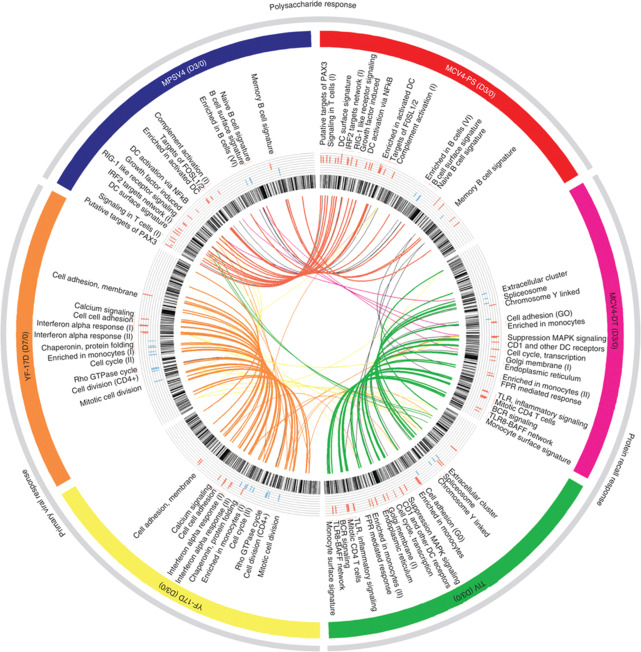
\includegraphics[width=0.6\textwidth]{pic/example.jpg}
    \caption{基因共表达网络示例\cite{example}}
\end{figure}

根据对表达出某疾病的许多样本的基因测序结果, 我们可以通过对同时出现的基因进行统计, 认为同时出现次数越多的基因可能会对该性状起阳性结果, 而出现次数较少的可以认为对该性状起阴性结果, 次数适中的认为是无关基因.

%我的表达可能不够合适……求大佬改改了, 介绍那段引用还没标

\section{数据来源以及初步分析}
\subsection{数据来源}
GEO数据库(Gene Expression Omnibus)是由美国国家生物信息中心(National Center for Biotechnology Information)提供维护服务的公共基因表达数据资源. 该数据库储存实验采集的原始数据并将其公开, 我们通过对GEO数据库上某个实验相关样本数据集系列(Series)进行分析, 就可以获得对基因间关系的深入认知, 以实现对疾病诱导原因的深入研究, 以及疾病的辅助治疗.

由于队伍成员设备运算能力的限制, 在处理单个系列时需要耗费大量时间(约193小时), 最后我们决定暂时只以GSE81089为数据来源, 计算非小细胞肺癌(non-small cell lung cancer, NSCLC)的基因关联网络.
\subsection{疾病介绍}
肺癌是世界上最常见的恶性肿瘤之一, 并且肺癌发生过程涉及的分子机制仍未被全部解开. 非小细胞肺癌\cite{wiki:NSCLC}包括鳞状细胞癌, 腺癌, 大细胞癌, 与小细胞癌相比其癌细胞生长分裂较慢, 扩散转移相对较晚, 对化疗相对不敏感. 非小细胞肺癌约占所有肺癌的85\%, 75\%的患者发现时已处于中晚期, 5年生存率很低. 而在非小细胞肺癌中, 病变部位的组织学分类决定了患者治疗的方式. 传统治疗只是针对病变部位的组织通过手术切除治疗,可以说治标不治本. 如果我们可以得知诱导NSCLC出现的基因是什么, 那么通过无效化这个基因就可以避免NSCLC的出现, 这样就形成了一种新的治疗方法.
\subsection{初步分析}
我们下载的数据是GEO上储存的经过实验团队初步处理的NSCLC的基因表达数据, 这是实验团队将199个来自seq的患病样本和142个正常样本进行基因测序比较后的结果. 经过实验团队的初步处理, 我们已经可以利用比较便利的方法读取数据, 而不是对实验原始数据进行文本处理. 

\section{假设与符号}
\subsection{假设}

\begin{enumerate}[I.]
    \item 基因与基因之间相对独立, 即全体样本中基因频率为定值
    \item 基因A与基因B之间的关系有三种: 正相关, 负相关和无关
    \item 视在实验选定的样本里出现次数多的基因对该疾病有促进作用
    \item 关于基因之间的关系, 我们认为有正相关, 负相关, 无关3种情况:
    \begin{enumerate}[i.]
        \item 认为正相关即相关系数$\rho \in [\alpha, 1]$
        \item 认为负相关为相关系数$\rho \in [-1,\alpha]$
        \item 认为无关为不属于上述二者的数据
    \end{enumerate}
\end{enumerate}

\subsection{符号}
\begin{table}[H]
    \centering
    \caption{符号说明}
    \begin{tabular}{r|l}
        \hline
        符号 & 意义\\
        \hline
        $\rho$ & 皮尔逊积矩相关系数\\
        $\alpha$ & 相关系数中的参数, 用于确定基因之间的关系\\
        $X/Y$ & 互相比较的两列数据, 即两个基因所对应的的所有样本上的数值\\
        \hline
    \end{tabular}
\end{table}



\section{问题分析}
\subsection{基因之间的联系表达}
基因之间的复杂的表达关系往往无法直接用数据表达, 因为基因A可能会对基因B起正相关作用, 对基因C起负相关, 而基因B和C对疾病都可能呈现正相关效果. 为了解释清楚这种关系, 我们将A,B,C与疾病之间的复杂关系描述为A与B, B与C, A与C之间的关系, 即相当于描述为网络中节点之间的关系.

由于基因之间的相对独立性, 我们可以在考虑AB之间的互相作用是忽略C

\subsection{等位基因}
等位基因指位于一对同源染色体相同位置上控制同一性状不同形态的基因.

在GEO数据库中, 等位基因会使用多个编号来标记, 即若A, B互为等位基因, 则A与B的ENSG编号是不同的. 这样就代表着在数据中会包含互补的数据(即等位基因). 这样的数据一般呈现A与B的出现频率相加约等于100\%的情况, 与我们认为的负相关情况类似, 所以我们不单独考虑等位基因对图中联系造成的影响, 而是将等位基因看做普通基因以参与计算.

\section{求解问题}
\subsection{皮尔逊积矩相关系数}
对于两组数据, 我们可以利用皮尔逊积矩相关系数\cite{wiki:pierxun}来求他们之间的相似程度. 

皮尔逊积矩相关系数(Pearson product-moment correlation coefficient,又称作PPMCC或PCCs, 文章中常用r或Pearson's r表示)是一种比较非中心化数据相似程度的一种方法, 该方法的特点在于得到的结果不受线性变换的影响, 即结果与数据的单位等无关.

下列三式可以求的不同的皮尔逊积矩相关系数, 我们在这里采用第一个式子.

\begin{equation}
    \rho_{X, Y}=\frac{\operatorname{cov}(X, Y)}{\sigma_{X} \sigma_{Y}}=\frac{E\left[\left(X-\mu_{X}\right)\left(Y-\mu_{Y}\right)\right]}{\sigma_{X} \sigma_{Y}}
\end{equation}

\begin{equation*}
    r=\frac{\sum_{i=1}^{n}\left(X_{i}-\overline{X}\right)\left(Y_{i}-\overline{Y}\right)}{\sqrt{\sum_{i=1}^{n}\left(X_{i}-\overline{X}\right)^{2}} \sqrt{\sum_{i=1}^{n}\left(Y_{i}-\overline{Y}\right)^{2}}}
\end{equation*}

\begin{equation*}
    r=\frac{1}{n-1} \sum_{i=1}^{n}\left(\frac{X_{i}-\overline{X}}{\sigma_{X}}\right)\left(\frac{Y_{i}-\overline{Y}}{\sigma_{Y}}\right)
\end{equation*}

由于基因的测量量单位FPKM(Fragments Per Kilobase of exon model per Million mapped fragments, 每千个碱基的转录每百万映射读取的fragments)与基因本身的规模有关, 所以数据库中得到的数据的均值由于基因的变化会发生较大的升降. 为了抵消这种对数据本身的拉伸对数据特征造成的破坏, 我们选择使用皮尔逊积矩相关系数这种更加本质的特征, 它反映了两组数据在线性上的相似性, 而非数据大小. 

皮尔逊积矩相关系数的取值范围在$[-1,1]$, 假设参数$\alpha$, 又假设$IV$中的内容, 只要选定了$\alpha$的值, 我们就可以将基因之间的关系区别为上述三种关系, 这样形成的矩阵无疑会对后续研究带来便利. $\alpha$的大小直接对结果造成影响, 根据文献\cite{wiki:pierxun}, 我们选取$\alpha=0.9$, 这样可以得到数据量不是特别巨大而且又可靠的联系矩阵.

我们利用python计算了GSE81089的数据, 所得到的矩阵可以在支撑材料里找到.

\subsection{结果的可视化}

仅仅获得相关系数的矩阵只是数据分析的一步, 要获得对于后续研究有所作用的直观图表, 我们需要将上述矩阵可视化. 基于假设$I$和$IV$, 我们可以认为基因在图中是点, 基因与基因之间的关系用不同颜色的线来代替. 如图\ref{1}, 其中红色的线表示该线所连接的一对基因之间的关系是正相关, 蓝色的线表示负相关. 无关的基因之间没有连线.
\begin{figure}[H]
    \centering
    \caption{简化的基因共表达网络}
    \label{1}
    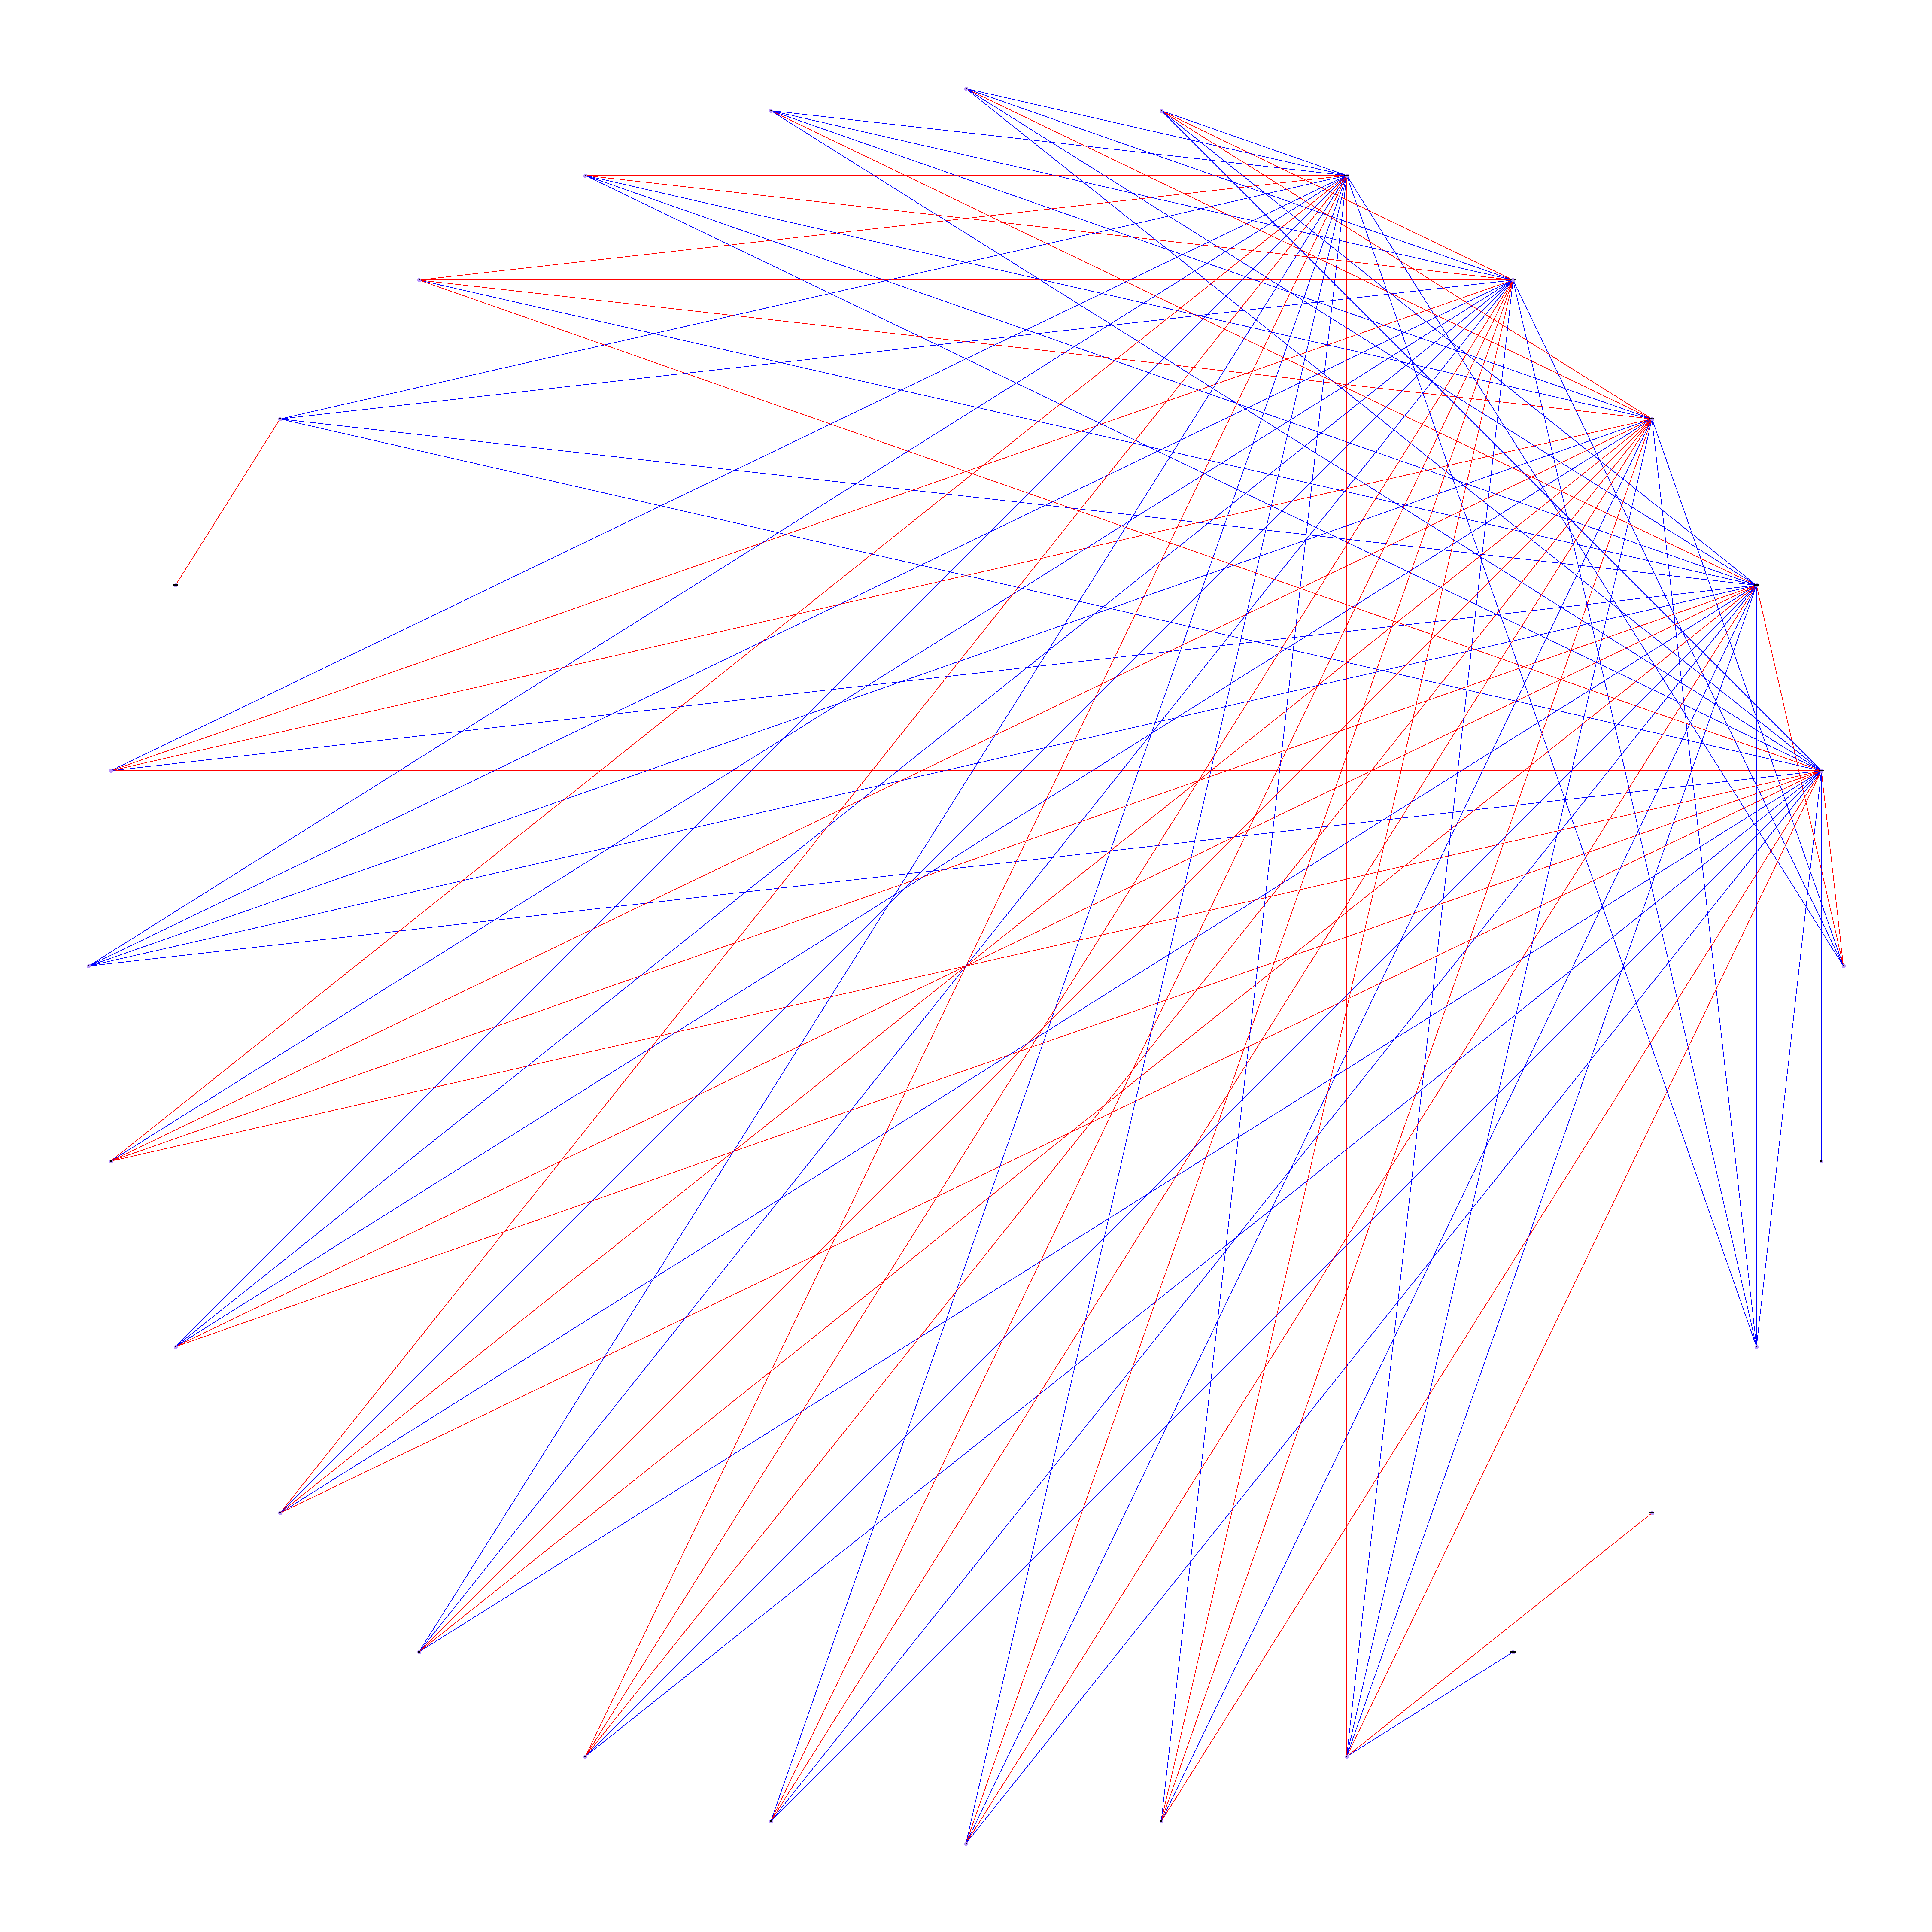
\includegraphics[width=0.8\textwidth]{pic/plot100.png}
\end{figure}

图\ref{1}只是整张图的一部分. 为了可以在论文里清晰的看出基因之间的联系, 我们舍弃了部分基因, 采取一部分基因来画出图\ref{1}. 完整的图可以在支撑材料里找到.

\newpage
\section*{结论}


\newpage
\section*{附录}

\bibliography{library}

\section*{支撑材料文件列表}

\dirtree{%
.1 /.
.2 \text{data}\DTcomment{从GEO下载的实验数据}.
.3 \text{FPKM-cufflinks.tsv}\DTcomment{GSE81089的实验数据}.
.2 \text{module}.
.3 \text{data-proceed.py}\DTcomment{处理数据得到相关系数矩阵脚本}.
.3 \text{math-model.ipynb}\DTcomment{数据可视化的jupyter文件}.
.3 \text{visualizeV1.py}\DTcomment{第一版本的数据可视化}.
.3 \text{visualizeV2.py}\DTcomment{第二版本的数据可视化}.
.2 \text{result}.
.3 \text{plot100.png}\DTcomment{取其中100条关系所绘制的图像}.
.3 \text{plotfull.png}\DTcomment{所有关系绘制的图像}.
.3 \text{plotmid.png}\DTcomment{其中一部分关系绘制的图像}.
.2 \text{readme}\DTcomment{文件列表}.
}
\end{document}
